\PassOptionsToPackage{unicode=true}{hyperref} % options for packages loaded elsewhere
\PassOptionsToPackage{hyphens}{url}
%
\documentclass[
]{article}
\usepackage{lmodern}
\usepackage{amssymb,amsmath}
\usepackage{ifxetex,ifluatex}
\ifnum 0\ifxetex 1\fi\ifluatex 1\fi=0 % if pdftex
\usepackage[T1]{fontenc}
\usepackage[utf8]{inputenc}
\usepackage{textcomp} % provides euro and other symbols
\else % if luatex or xelatex
\usepackage{unicode-math}
\defaultfontfeatures{Scale=MatchLowercase}
\defaultfontfeatures[\rmfamily]{Ligatures=TeX,Scale=1}
\fi
% use upquote if available, for straight quotes in verbatim environments
\IfFileExists{upquote.sty}{\usepackage{upquote}}{}
\IfFileExists{microtype.sty}{% use microtype if available
	\usepackage[]{microtype}
	\UseMicrotypeSet[protrusion]{basicmath} % disable protrusion for tt fonts
}{}
\makeatletter
\@ifundefined{KOMAClassName}{% if non-KOMA class
	\IfFileExists{parskip.sty}{%
		\usepackage{parskip}
	}{% else
		\setlength{\parindent}{0pt}
		\setlength{\parskip}{6pt plus 2pt minus 1pt}}
}{% if KOMA class
	\KOMAoptions{parskip=half}}
\makeatother
\usepackage{xcolor}
\IfFileExists{xurl.sty}{\usepackage{xurl}}{} % add URL line breaks if available
\IfFileExists{bookmark.sty}{\usepackage{bookmark}}{\usepackage{hyperref}}
\hypersetup{
	pdfborder={0 0 0},
	breaklinks=true}
\urlstyle{same}  % don't use monospace font for urls
\setlength{\emergencystretch}{3em}  % prevent overfull lines
\providecommand{\tightlist}{%
	\setlength{\itemsep}{0pt}\setlength{\parskip}{0pt}}
\setcounter{secnumdepth}{-2}
% Redefines (sub)paragraphs to behave more like sections
\ifx\paragraph\undefined\else
\let\oldparagraph\paragraph
\renewcommand{\paragraph}[1]{\oldparagraph{#1}\mbox{}}
\fi
\ifx\subparagraph\undefined\else
\let\oldsubparagraph\subparagraph
\renewcommand{\subparagraph}[1]{\oldsubparagraph{#1}\mbox{}}
\fi

\usepackage{graphicx}
\usepackage{float}

% set default figure placement to htbp
\makeatletter
\def\fps@figure{htbp}
\makeatother


\date{}

\begin{document}
	
	\hypertarget{cis-5520-project-proposal}{%
		\section{CIS 5520 Project proposal}\label{cis-5520-project-proposal}}
	
	\begin{itemize}
		\item
		Group members:
		Steven Galban, Huynh Quynh Anh
		\item
		Github ids:
		sgalban, hqanhh
		\item
		Project title: Puzzle Solver
	\end{itemize}
	
	\hypertarget{overall-goal}{%
		\subsection{1. Overall goal}\label{overall-goal}}
	
	Consider the family of number puzzles containing games such as Sudoku, Kakuro, and Magic Squares. While they all have different rules, at their core, they can all be modeled as a grid of numbers subject to certain constraints. This project aims to take advantage of these similarities, generalizing these puzzles into a common framework, and then using that framework to create a general puzzle solver.
	Specifically, the goal of this project is to create a domain-specific language, Puzzle, that can be used to describe a family of similar grid-based number puzzles (including Sudoku, Kakuro, Magic Squares, and more), and then write a small Haskell library with three primary functions: \begin{enumerate}
		\item To parse this domain-specific language into a Haskell persistent data structure.
		\item To convert puzzles back into Puzzle code.
		\item To determine the solution of an unsolved puzzle (or indicate that no such valid solution exists).
	\end{enumerate} 
	This library will be complete with a command-line interface from which users can perform all the functionality described above.
	
	\hypertarget{use-case}{%
		\subsection{2. Use case}\label{use-case}}
	
	The use cases for this library are fairly straightforward. For example, from the command-line interface, a user can load a Puzzle file via its filepath, which parses the puzzle and loads it into memory. Once the puzzle is loaded, the user can then modify it, or solve it. For example, suppose the user wants to solve the following 4x4 Sudoku puzzle:
	\begin{figure}[H]
		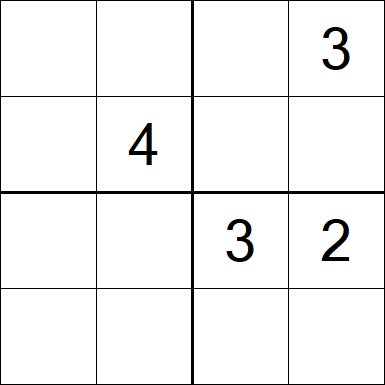
\includegraphics[width=4cm]{sudoku}
	\end{figure}
	To solve this puzzle, the user would first load the following Puzzle code: \begin{verbatim}
grid(4, 4) {
    # Each row has unique entries
    repeat(0, 3) {
        constraint unique(1 to 4) in row $0
    }
    # Each column has unique entries
    repeat(0, 3) {
        constraint unique(1 to 4) in col $0
    }
    # Each box has unique entries
    repeat(0, 3) {
        constraint unique(1 to 4) in subgrid((($0 % 2) * 2, ($0 // 2) * 2), 2, 2)
    }
    init cell(0, 4) with 3
    init cell(1, 1) with 4
    init cell(2, 2) with 3
    init cell(2, 3) with 2
} 
	\end{verbatim}
	
	then simply use the solve command. Other types of puzzles that can be modeled by Puzzle code, and are therefore compatible with the library, include but are not limited to, Kakuro, Magic Squares, KenKen, Killer Sudoku, and Futoshiki.
	\hypertarget{project-architecture}{%
		\subsection{3. Project architecture}\label{project-architecture}}
	
	This project covers multiple separate domains, and lends itself well to being organized over several modules:\begin{enumerate}
		\item \textbf{Puzzle}:\\
		At the core of this project is the \texttt{Puzzle} model, which represents both an unsolved puzzle, and parsed Puzzle code. That is, it describes the shape of the grid, its initial values, and all the constraints the puzzle is subject to. This module exposes a function that validates structure of a puzzle, i.e. to ensure that every cell of a puzzle either has an initial value, or is subject to at least one constraint. \texttt{Puzzle} will be an instance of \texttt{PrettyPrint}, its string representation being Puzzle code that could be used to describe the puzzle. This module will also contain a separate method that converts a puzzle into an ASCII representation of the grid, which will be useful for debugging and visualization.\\
		Additionally, this module will contain the \texttt{PuzzleSolution} type, which is essentially a pair containing a \texttt{Puzzle}, and a mapping from cell coordinates to values used to fill the cells. This model represents total and partial solutions to the puzzle.
		\item \textbf{PuzzleSolver}:\\
		This module handles solving the puzzle. Its primary purpose is to expose two functions: one that solves a puzzle, and one that validates a full or partial solution.
		
		The \texttt{solve} function will accept a \texttt{Puzzle} as input, and output an \texttt{Maybe PuzzleSolution}, containing a complete valid solution (or \texttt{Nothing}, if no valid solution exists). Note that solving many of the puzzles described by this DSL are NP-Complete problems, so the solver will not be particularly fast for larger puzzles, but the implementation may use various techniques to reduce the runtime as much as feasibly possible.
		
		The \texttt{validate} function takes a \texttt{PuzzleSolution} and returns true if and only if the solution does not violate any of the puzzle's constraints. A fully solved puzzle is a \texttt{PuzzleSolution} containing a value for every cell.
		
		\item \textbf{PuzzleParser}:\\
		The parser module exposes only one function, \texttt{parsePuzzle}, which accepts a filename for a Puzzle file as input and parses its contents into an \texttt{Either Puzzle}, where the \texttt{Left} case represents parsing errors.
		
		\item \textbf{PuzzleCLI}:\\
		The CLI module ties the other modules in this project together, allowing users to access the above functionality without writing any of their own Haskell code. Specifically, this module will allow users to load puzzles from the Puzzle code files, solve those puzzles, modify them, and print them in various formats.
	\end{enumerate}
	
	\hypertarget{testing}{%
		\subsection{4. Testing}\label{testing}}
	
	Most of the testing for the project will be focused on the Puzzle solver, as valid solutions have some nice properties that lend themselves well to QuickCheck. For example: \begin{itemize}
		\item If the \texttt{solve} function outputs a \texttt{Just PuzzleSolution}, the solution should be valid.
		\item If a puzzle has a valid structure and an empty solution, its solution is valid.
		\item If any cell from a valid (partial) solution is cleared, the result should still be valid.
		\item if any blank cell from an invalid (partial) solution is added, the result should still be invalid.
	\end{itemize}
	Additionally, the parser module can contain at least one roundtrip QuickCheck property, ensuring that converting a \texttt{Puzzle} into Puzzle code and parsing it back results in an equivalent \texttt{Puzzle}.
	Furthermore, several sample puzzles and their solutions could be hard-coded (similarly to homework 5), which could be used to unit test both the solver and the parser.
	
\end{document}
